\section{Результаты работы тренировки}

\subsection{Вариант 0}

По умолчанию выставлен задач планирования --- фиксированный объем рессурсов.

\begin{figure}[ht!]
	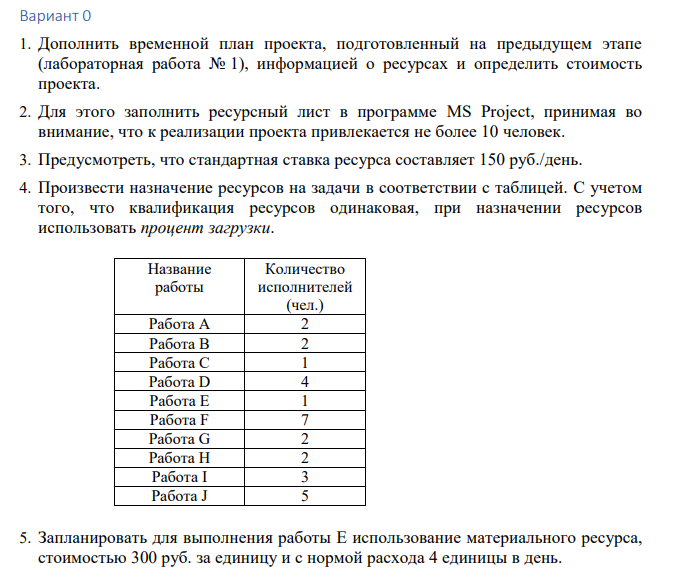
\includegraphics[width=0.75\linewidth]{assets/images/image_2024-02-27_09-41-29.png}
	\label{fig:r2}
	\caption{Задание тренировки}
\end{figure}
\FloatBarrier


\begin{figure}[ht!]
	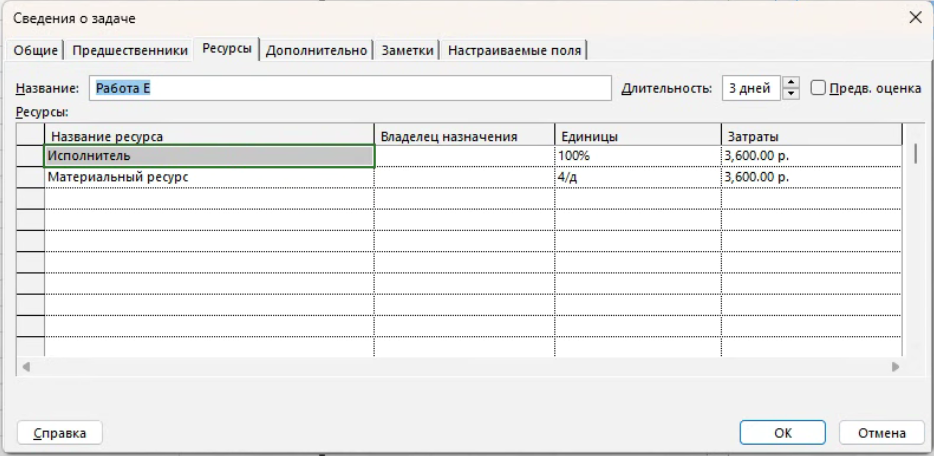
\includegraphics[width=\linewidth]{assets/images/Screenshot 2024-02-27 at 14.25.08.png}
	\label{fig:r2}
	\caption{Установка материального рессурса}
\end{figure}
\FloatBarrier

\begin{figure}[ht!]
	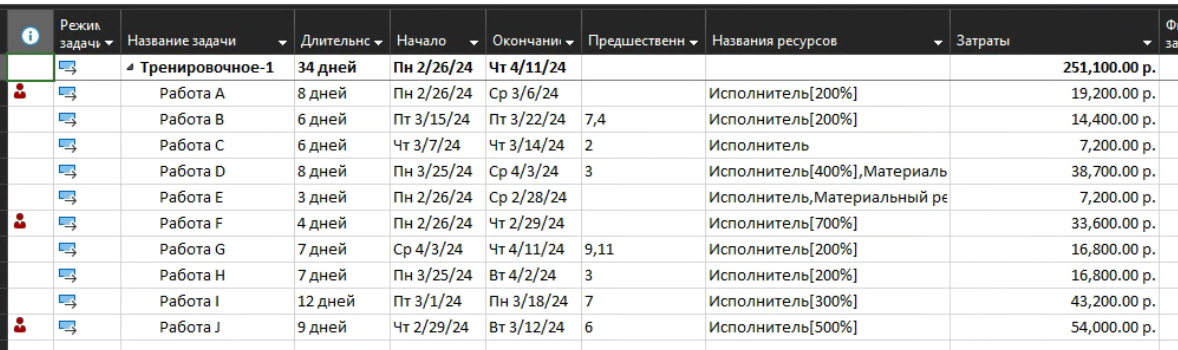
\includegraphics[width=\linewidth]{assets/images/Screenshot 2024-02-27 at 14.27.24.png}
	\label{fig:r2}
	\caption{Резульатат тренировочного задания}
\end{figure}
\FloatBarrier

\section{Результаты работы второй лабораторной работы}

\subsection{Создание списка ресурсов}

\begin{figure}[ht!]
	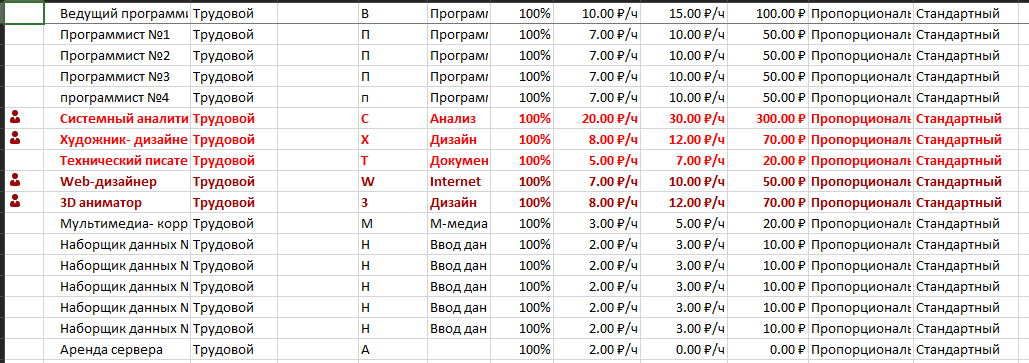
\includegraphics[width=0.75\linewidth]{assets/images/image_2024-02-27_09-33-23.png}
	\label{fig:r2}
	\caption{Ресусры}
\end{figure}
\FloatBarrier

\subsection{Назанчение ресурсов задачам}

\begin{figure}[ht!]
	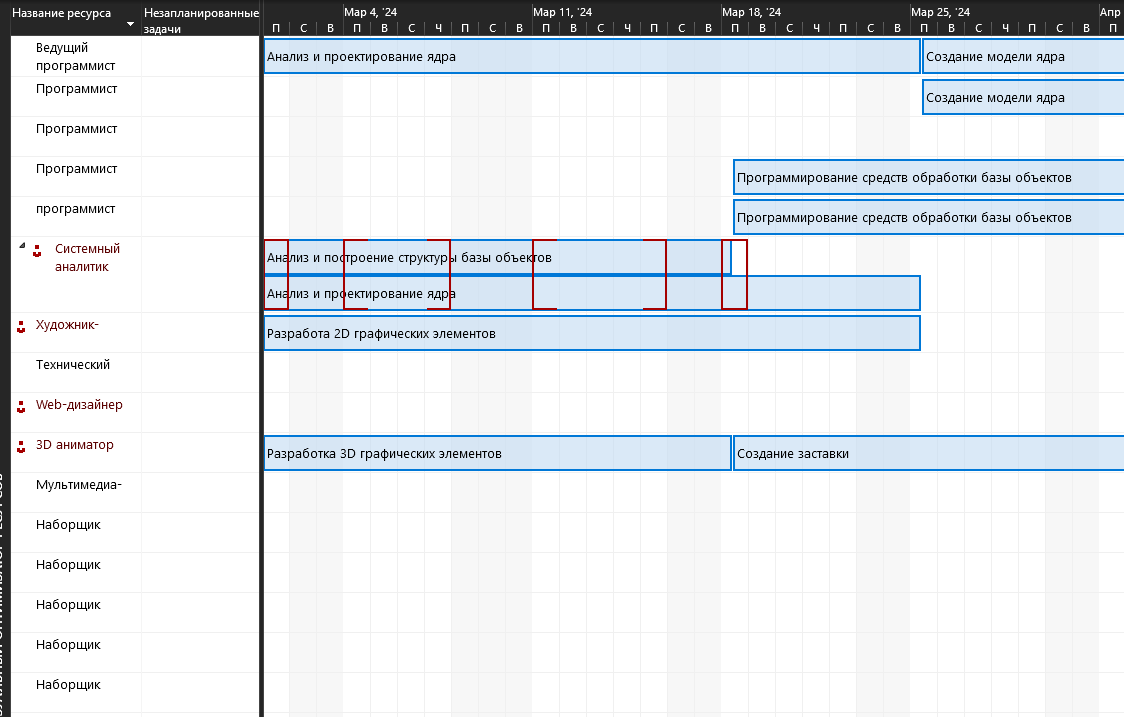
\includegraphics[width=0.75\linewidth]{assets/images/image_2024-02-27_09-35-16.png}
	\label{fig:r2}
	\caption{Ресусры}
\end{figure}
\FloatBarrier

Видно, что у художника-дизайнера задачи (разработка дизайна руководства и разработка дизайна сайта) накладываются друг на друга и он не успевает их выполнить.
У технического писателя --- написание руководства пользователя и создание справочной системы.
У системного аналитика --- анализ и построение структуры объектов, и анализ и проектирование ядра.

\begin{figure}[ht!]
	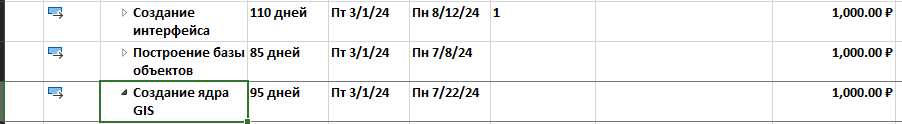
\includegraphics[width=0.75\linewidth]{assets/images/image_2024-02-27_09-35-44.png}
	\label{fig:r2}
	\caption{Ресусры}
\end{figure}
\FloatBarrier

Назначен аренда сервера как трудовой ресурс, так как стоимость его использования пропорционально времени.
Для него был назначен 24 часовой календарь. Стоитмость использования за весь проект 6198 рублей.

\subsection{Анализ затрат по группам ресурсов}

\begin{figure}[ht!]
	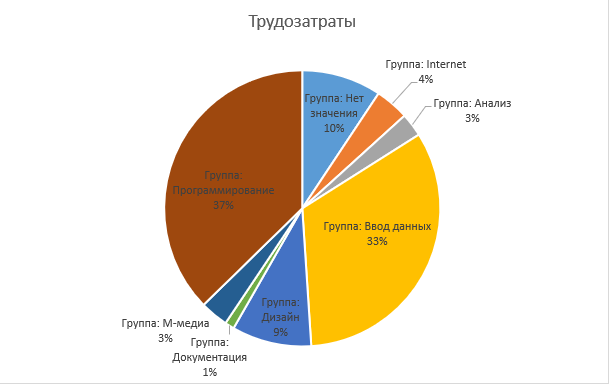
\includegraphics[width=0.75\linewidth]{assets/images/image_2024-02-27_11-32-35.png}
	\label{fig:r2}
	\caption{Затраты}
\end{figure}
\FloatBarrier

\begin{figure}[ht!]
	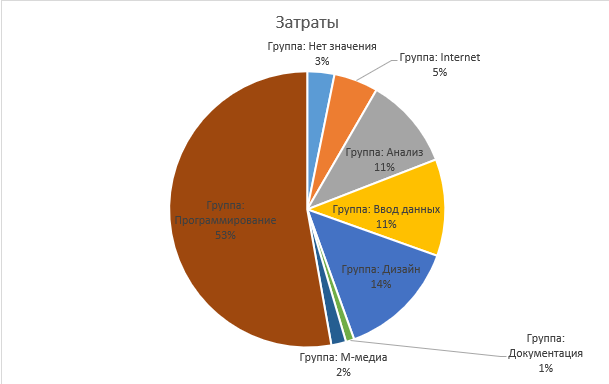
\includegraphics[width=0.75\linewidth]{assets/images/image_2024-02-27_11-33-30.png}
	\label{fig:r2}
	\caption{Трудозатраты}
\end{figure}
\FloatBarrier

\subsection*{Вывод}

Согласно диаграммам, можно сделать вывод, что наиболее затратная работа прораммистов, сервера и анализа.
При этом наборщик данных выполняют 25 процентов работы и затрачивают 10 процентов бюджета.
У программистов и аналитиков наибольшее соотношение затарат к трудозатратам.
Обратная ситуация наблюдается у сервера.